\documentclass[11pt]{extarticle}

\usepackage[english,french]{babel}
\usepackage[utf8]{inputenc}
\usepackage{url}
\usepackage[T1]{fontenc}
\usepackage{booktabs}
\usepackage{enumitem}
\usepackage{graphicx}
\usepackage{pifont}
\usepackage{makecell}
\setcellgapes{1pt}
\usepackage{placeins}
\usepackage{subcaption}
\usepackage{pgfplots}
\usetikzlibrary{calc}
\pgfplotsset{compat=1.18}
\usepackage[margin=1in]{geometry}
\usepackage[colorlinks=true, allcolors=blue]{hyperref}
\usepackage{amsmath}
\usepackage{pgfplotstable}
\usepackage{amsfonts}
\usetikzlibrary{backgrounds}

\title{
    \hspace*{-12cm}
    \vspace*{1cm}
    \protect\\
    \vspace*{1cm}
    \textbf{Long Term Memory Processes Using Hurst Estimation}
}

\author{Remiat Alexandre}

\date{\today}

\graphicspath{{img/}}

\xdefinecolor{kblue}{RGB}{0,38,69}
\xdefinecolor{korange}{RGB}{255,128,89}
\xdefinecolor{kgray}{RGB}{47,108,130}
\xdefinecolor{kgreen}{RGB}{102,143,72}


\begin{document}

\selectlanguage{english}

\maketitle

\vspace{1.5cm}
{
  \hypersetup{linkcolor=black}
  \tableofcontents
  % \listoffigures
}

\newpage


\section*{Abstract}

This paper presents a study on long-term memory processes in financial time series using Hurst estimation methods, specifically the traditional R/S statistic (Rescaled Range analysis) and the Modified R/S statistic.
We analyze the long-term memory properties of five major stock market indices: S\&P 500 (GSPC), FTSE 100 (FTSE), SBF 250 (SBF250), TOPIX (TOPX), and Toronto Stock Exchange 300 (GSPTSE) using daily returns data spanning from January 2, 1995, to December 31, 2024.

The R/S statistic and the Modified R/S statistic are computed to determine the presence of long-range dependence in the time series data. The Hurst exponent, derived from both statistics, is used to characterize the memory behavior of the series.

The results indicate that, except for GSPC, all indices exhibit short-term memory or randomness with Hurst exponents below the critical threshold of 1.620.
Specifically, the Hurst exponent for the GSPC index exceeds 1.620, indicating the presence of long-term memory (persistent behavior).
These findings suggest that certain stock markets, like the US stock market represented by GSPC, may exhibit more pronounced long-term memory effects compared to others.


\newpage

\section{Introduction}

The Hurst exponent is a key measure in the study of time series data, used primarily to analyze the long-term memory and self-similarity of stochastic processes. First introduced by the British hydrologist Harold Hurst in the 1950s to study river flow data, the Hurst exponent has since found widespread application in various fields, including finance, physics, and environmental science. The exponent provides insights into the persistence or mean-reversion behavior of a time series: a value greater than 0.5 indicates long-range dependence and persistence, while a value less than 0.5 suggests mean-reverting behavior.

The most commonly used method to estimate the Hurst exponent is the Rescaled Range (R/S) analysis, introduced by Hurst and later refined by Mandelbrot. However, the traditional R/S statistic has limitations, particularly in its sensitivity to short-term memory effects, which can obscure long-range dependence in the data. To address these issues, Lo (1991) proposed the Modified R/S statistic, which improves the estimation of the Hurst exponent by accounting for short-term autocorrelation.

This paper presents an analysis of time series data using both the traditional R/S statistic and the Modified R/S statistic, with a focus on their ability to detect long memory in financial data. We apply these methods to a range of stock market indices and examine the significance of the Hurst exponent in characterizing market dynamics. Additionally, we discuss the critical values for the Modified R/S test, based on Lo’s (1991) table, to help identify whether a series exhibits long memory behavior.

Through this analysis, we aim to highlight the advantages of the Modified R/S statistic in overcoming the limitations of the traditional R/S method, providing a more robust framework for studying time series with long memory. This is particularly valuable in the context of financial markets, where long memory and fractal-like behavior are often observed.



\section{Methods}

\subsection{Fractional Brownian Motion}

Fractional Brownian motion (fBm) is a generalization of standard Brownian motion that introduces dependence in increments,
making it suitable for modeling processes with memory effects. It is a continuous-time Gaussian process \( X_H(t) \) H corresponds
to the Hurst exponent and \( H \in [0, 1] \) with the following properties:

\begin{itemize}
    \item \( X_H(0) = 0 \).
    \item The increments \( X_H(t) - X_H(s) \) follow a normal distribution with mean zero and variance:
    \begin{equation}
        \mathbb{E} \left[ (X_H(t) - X_H(s))^2 \right] = \sigma^2|t - s|^{2H},
    \end{equation}
    where \( H \) is the Hurst exponent.
    \item The process exhibits self-similarity, meaning that for any scaling factor \( c \), \( c \in \mathbb{R}^+ \), the rescaled process satisfies:
    \begin{equation}
        X_H(ct) \overset{d}{=} c^H X_H(t).
    \end{equation}
    \item When \( H = 0.5 \), fBm reduces to classical Brownian motion.
    \item For \( H > 0.5 \), the process exhibits long-term positive autocorrelation, meaning that an increase in the past tends to be followed by further increases.
    \item For \( H < 0.5 \), the process has anti-persistent behavior, where an increase in the past is more likely to be followed by a decrease.
\end{itemize}

The covariance function of fBm is given by:

\begin{equation}
    C_H(t_1, t_2) = \frac{\sigma^2}{2} \left( t_1^{2H} + t_2^{2H} - |t_1 - t_2|^{2H} \right),
    \label{eq:fbm_covariance}
\end{equation}

which accounts for the dependence structure of the process. The Hurst exponent \( H \) plays a critical role in determining the smoothness and correlation properties of fBm:

\begin{itemize}
    \item \textbf{For small \( H \) values} (\( H < 0.5 \)), the process is highly erratic, with rapid changes and weak memory effects.
    \item \textbf{For large \( H \) values} (\( H > 0.5 \)), the trajectory becomes smoother, and the process exhibits long-range dependence.
\end{itemize}

Fractional Brownian motion is widely used in finance, telecommunications, and physics to model phenomena exhibiting memory effects and self-similarity, such as stock market fluctuations, internet traffic, and geological formations.


\subsection{Simulation of Fractional Brownian Motion}

To generate the fractional Brownian motion (fBm), we use a Cholesky decomposition-based approach. The covariance matrix of fBm is given by \eqref{eq:fbm_covariance}:

where \( H \) is the Hurst exponent, which determines the degree of long-term dependence in the process.

The steps of the simulation are as follows:
\begin{enumerate}
    \item Define a time grid of \( N \) points between \( 0 \) and \( T \).
    \item Compute the covariance matrix using the formula above.
    \item Apply Cholesky decomposition to obtain a lower triangular matrix \( L \).
    \item Generate a vector \( W \) of standard normal random variables.
    \item Obtain the fBm path by computing \( X = L W \).
\end{enumerate}

The params used for this simulation are N = 1000, T = 1, and Hurst exponents \( H = 0.2, 0.3, 0.5, 0.6, 0.8 \), the number
of lag for the autocorrelation is 40.

\begin{figure}[!ht]
    \centering
    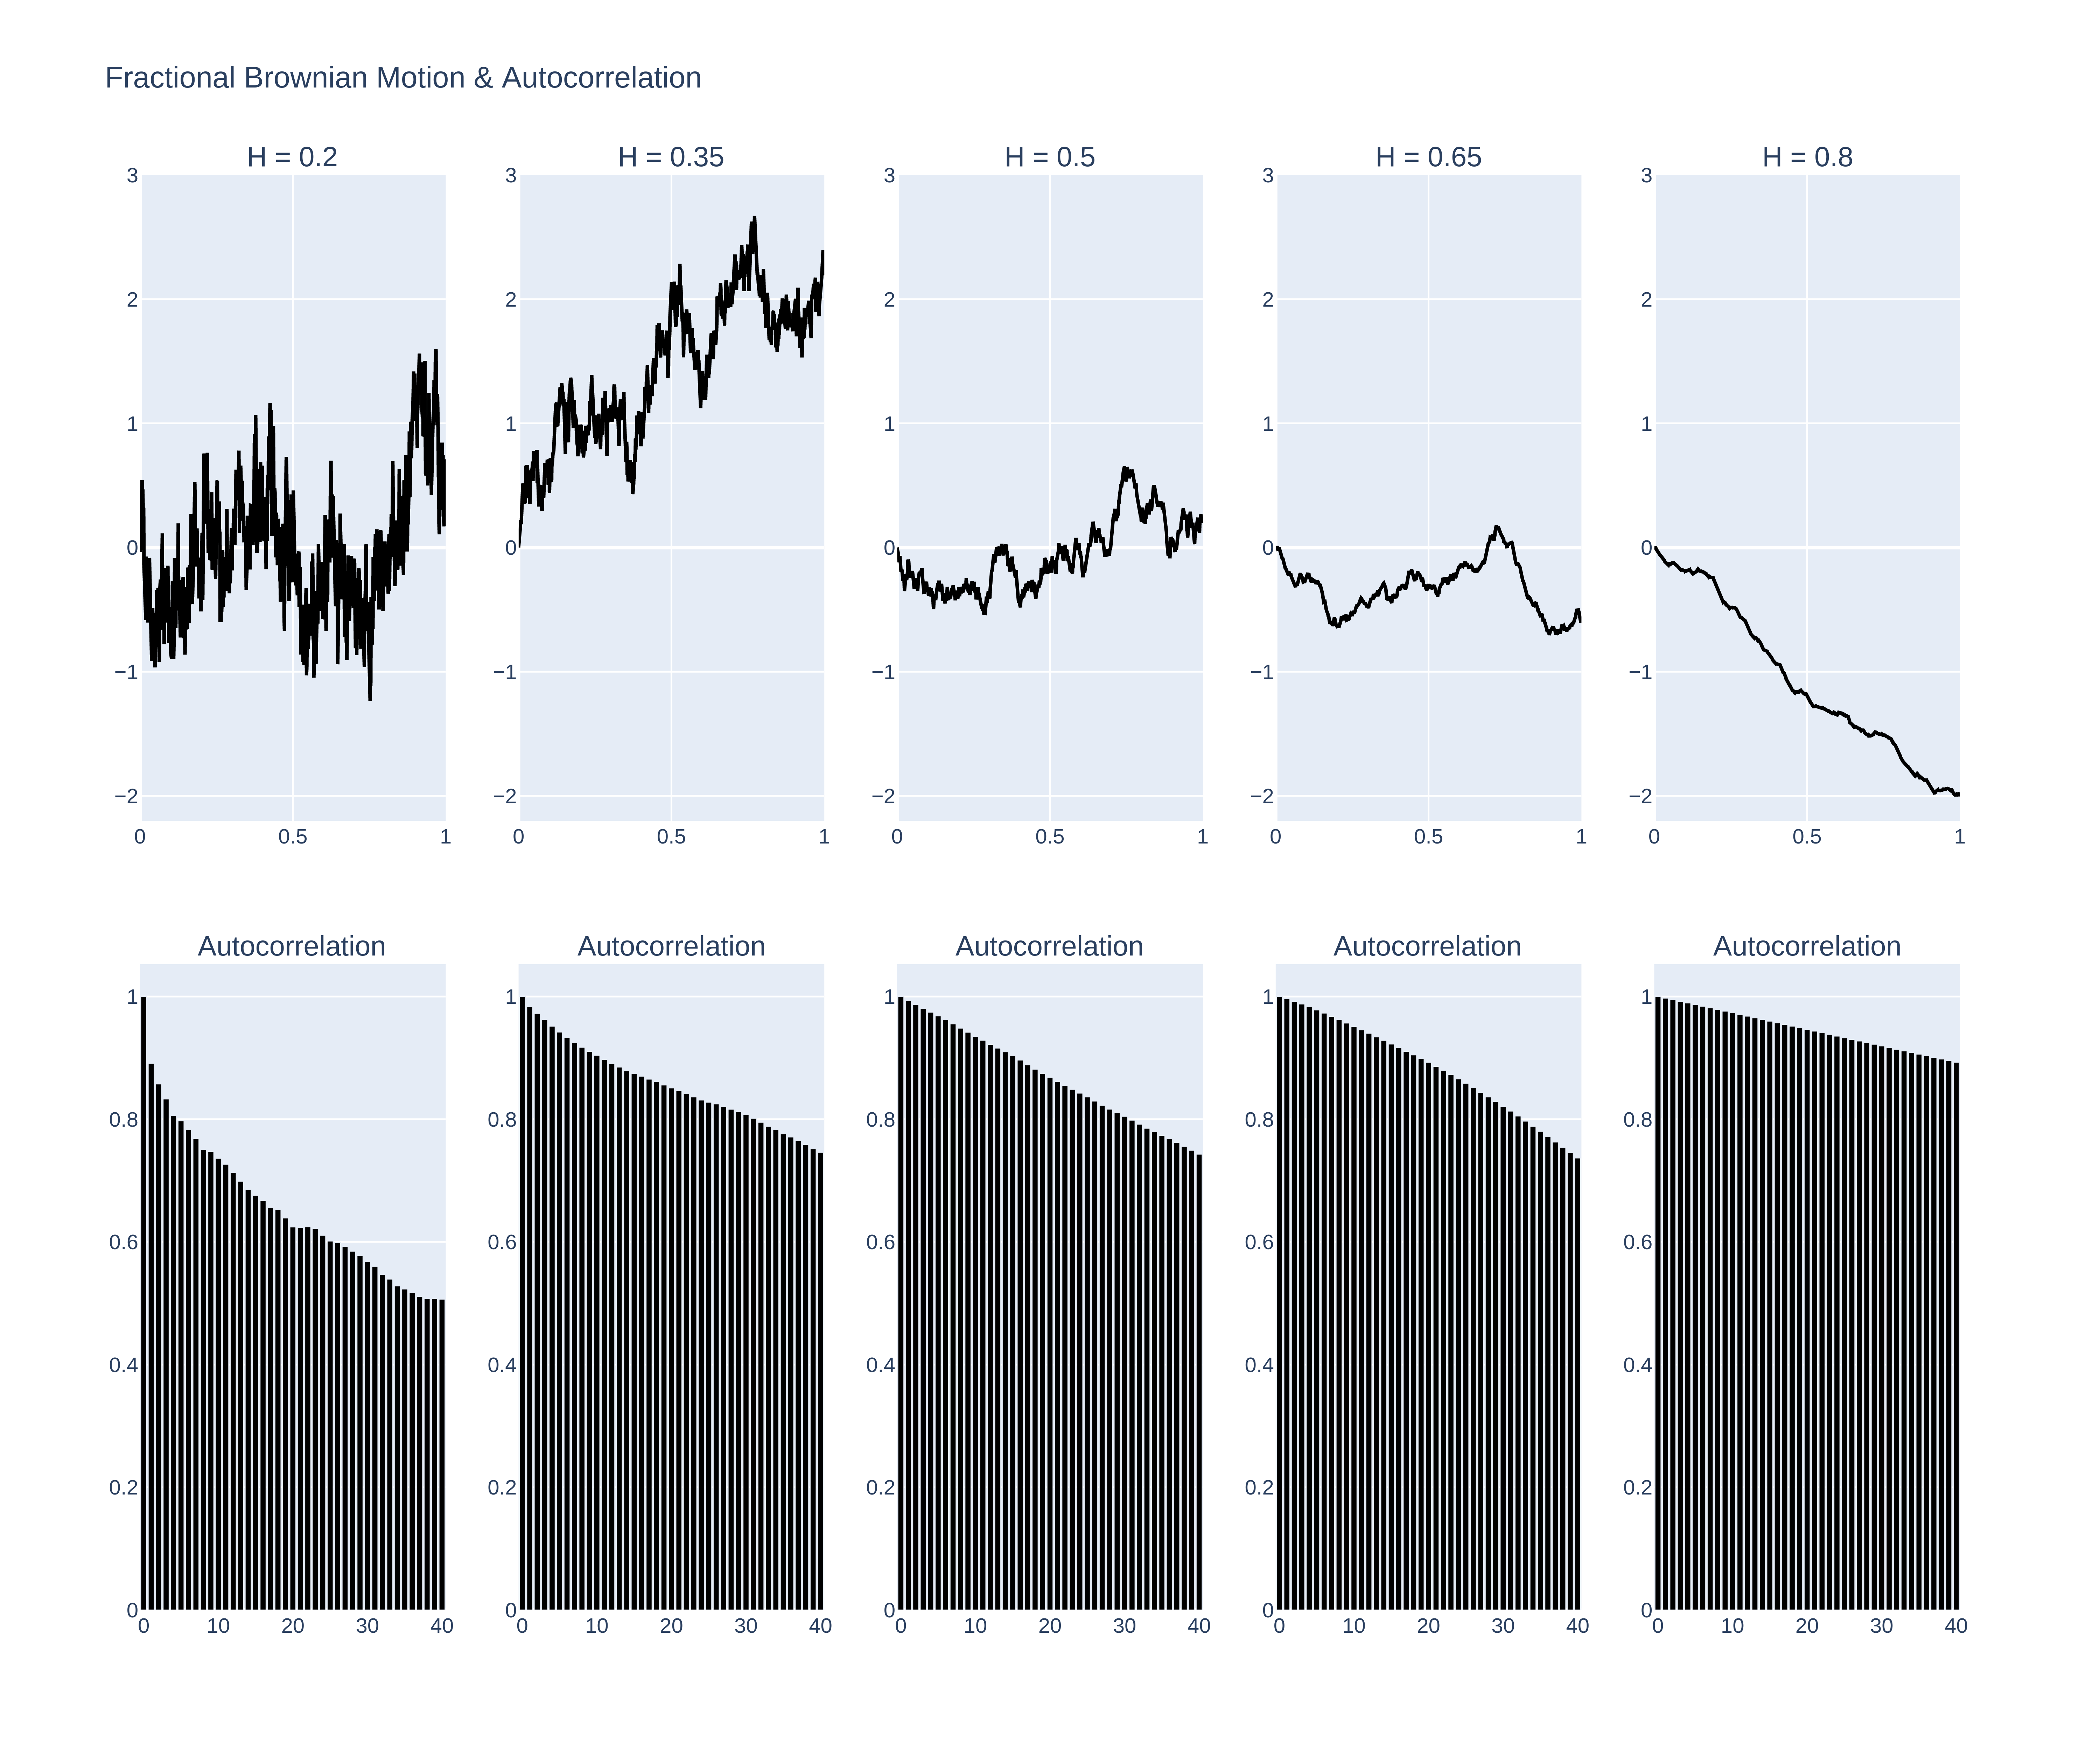
\includegraphics[width=0.8\textwidth]{img/fdm_autocorr}
    \caption{Simulation of Fractional Brownian Motion with different Hurst exponent and its autocorrelation function.}
    \label{fig:fbm_autocorr}
\end{figure}

\FloatBarrier

The behavior of the fractional Brownian motion (fBm) varies significantly with the Hurst exponent \( H \).

When \( H \) is small (close to 0), the fBm exhibits high local variability, resulting in a highly granular trajectory with frequent fluctuations. The autocorrelation of increments decays rapidly, indicating that future values are weakly influenced by past values. This suggests a short-memory process, similar to standard Brownian motion.

As \( H \) increases, the autocorrelation decays more slowly, meaning that past values have a more significant impact on future values. This introduces a form of long-term dependence, where the process exhibits persistent trends. Consequently, the fBm trajectory appears smoother, with larger coherent movements and fewer abrupt changes.

In summary, a lower \( H \) leads to a more irregular and noisy path, characteristic of short-memory processes, while a higher \( H \) results in a smoother trajectory with stronger persistence.

\subsection{Hurst Exponent Calculation}
\subsection{R/S and Modified R/S Analysis}
The R/S (Rescaled Range ) analysis , introduced by Hurst and developed in various works by Mandelbrot, is certainly the most well-known method for estimating the Hurst exponent $H$. This statistic is defined as the range of the partial sums of deviations from the mean of a time series divided by its standard deviation. Consider a time series $Y_t$, $t = 1, ..., T$, with mean $\bar{Y}$. The range $R$ is defined as:

\[
R = \max_{1 \leq j \leq T} \left( Y_j - \bar{Y} \right) - \min_{1 \leq j \leq T} \left( Y_j - \bar{Y} \right)
\]

The R/S statistic is then computed by dividing the range by the standard deviation $s_T$ of the series:

\[
Q_T = \frac{R}{s_T} = \frac{\max_{1 \leq j \leq T} \left( Y_j - \bar{Y} \right) - \min_{1 \leq j \leq T} \left( Y_j - \bar{Y} \right)}{s_T}
\]

The R/S statistic, $Q_T$, is always positive. In various papers, Mandelbrot and Wallis (1969e), Mandelbrot (1973), and Mandelbrot and Taqqu (1979) have emphasized the superiority of R/S analysis over more traditional methods of detecting long memory, such as autocorrelation studies, variance ratio tests, and spectral analysis. Mandelbrot and Wallis (1968) show that R/S analysis can detect long memory even in highly non-Gaussian time series. Mandelbrot and Wallis (1969d) further note that, unlike spectral analysis which only detects periodic cycles, the R/S statistic can detect non-periodic cycles. Finally, Mandelbrot and Wallis (1969e) demonstrate that the R/S statistic is independent of the marginal distribution.

The R/S analysis leads to the Hurst exponent, where $T$ is the number of observations in the series.

\subsection{Modified R/S Analysis}
The Modified R/S statistic, denoted by $\tilde{Q}_T$, is defined as:

\[
\tilde{Q}_T = \frac{R}{\hat{\sigma}_T(q)}
\]

where

\[
\hat{\sigma}_T(q) = \sqrt{\frac{1}{T} \sum_{j=1}^{T} (Y_j - \bar{Y})^2 + \frac{2}{T} \sum_{j=1}^{T} w_j(q) \left[ \sum_{i=j+1}^{T} (Y_i - \bar{Y})(Y_{i-j} - \bar{Y}) \right]}
\]

and

\[
w_j(q) = 1 - \frac{j}{q + 1}
\]

This statistic differs from the traditional R/S statistic only by its denominator. In the presence of autocorrelation, the denominator does not only represent the sum of the variances of the individual terms, but also includes autocovariances.
These are weighted according to lags $q$, with the weights $w(q)$ suggested by Newey and West (1987). Moreover, Andrews (1991) proposed a rule for choosing $q$:

\[
q = \left[ k_T \right] \quad \text{where} \quad k_T = \left( \frac{3T}{2} \right)^{1/3} \left( \frac{2 \rho_1}{1 - \rho_1} \right)^{2/3}
\]

where $[k_T]$ is the integer part of $k_T$, and $\rho_1$ is the first-order autocorrelation coefficient.

Unlike the classical R/S analysis, the limiting distribution of the Modified R/S statistic is known, and the statistic $V$, defined by

\[
V = \frac{\tilde{Q}_T}{\sqrt{T}},
\]

converges to the range of a Brownian bridge over the unit interval. It is therefore possible to perform a statistical test for the null hypothesis of short memory against the alternative hypothesis of long memory by referring to the critical value table provided by Lo (1991).

\subsection{Critical Value Table from Lo (1991)}
The critical values for the Modified R/S test are provided in the table below. These values are used to assess whether the series exhibits long memory behavior based on the Modified R/S statistic.

\begin{table}[ht!]
\centering
\begin{tabular}{|c|c|c|}
\hline
\textbf{Significance Level} & \textbf{Critical Value (Modified R/S Statistic)} \\
\hline
0.005 & 2.098\\
0.05 & 1.747\\
0.10 & 1.620\\

\hline
\end{tabular}
\caption{Critical values for the Modified R/S Statistic (Lo, 1991)}
\end{table}



\section{Data}

The data used in this analysis consists of the historical closing prices of five major stock market indices: the S\&P 500 (GSPC), FTSE 100 (FTSE), SBF 250 (SBF250), TOPIX (TOPX), and the Toronto Stock Exchange 300 (GSPTSE).
The data spans the period from January 2, 1995, to December 31, 2024, and was downloaded from Yahoo Finance.

For each index, the closing price time series was transformed using the natural logarithm to obtain a series of log returns.
These log returns were then used to calculate the R/S and Modified R/S statistics and estimate the Hurst exponent.
The purpose of using this data is to evaluate the long-term memory properties of financial markets, which can indicate persistence or mean-reversion in market behavior.

Additionally, a stationarity test was conducted on the log return series using the Augmented Dickey-Fuller (ADF) test.
The results indicated that all series were non-stationary, suggesting the presence of unit roots. To address this, the series were differenced once, after which they exhibited stationarity.
This step ensures that the analysis of long-term memory is conducted on properly transformed data, free from non-stationary distortions.

\section{Results}


The following table summarizes the results of the R/S statistic, Modified R/S statistic, and the estimated Hurst exponents for each of the five indices analyzed: \\

\begin{table}[h!]
    \centering
    \pgfplotstabletypeset[
        col sep=comma,
        header=true,
        string type,
        every head row/.style={before row=\hline, after row=\hline},
        every last row/.style={after row=\hline},
        columns/Ticker/.style={column name=Ticker, string type},
        columns/R/S Statistic/.style={column name=R/S Statistic, fixed, precision=2},
        columns/Hurst Exponent (RS)/.style={column name=Hurst Exponent (RS), fixed, precision=3},
        columns/Modified Hurst Exponent/.style={column name=Modified Hurst Exponent, fixed, precision=3},
        columns/Critical Value/.style={column name=Critical Value, fixed, precision=3},
        columns/Long Memory/.style={column name=Long Memory}
    ] {data/hurst_results.csv}
    \caption{Results for R/S and Modified R/S Statistics, Hurst Exponent, and Long Memory 10\%.}
    \label{tab:hurst_results}
\end{table}

\FloatBarrier


Based on the results obtained from applying the traditional R/S method, all the series appear to exhibit long-term memory,
as the Hurst exponents are consistently greater than 0.5. However, the asymptotic distribution of this statistic is unknown,
which prevents us from determining whether the estimated Hurst exponent is significantly greater than 0.5. This issue can be
addressed by using the modified R/S method. In this case, we simply compare the estimated values of the statistic V to the
critical values provided by Lo (1991), which are 1.620 and 1.747 for the 10\% and 5\% significance levels, respectively,
in the case of a one-tailed test. It is observed that only one serie actually exhibit persistence: the returns of the S\&P 500 stock indices (US).
For all other series, despite the Hurst exponent being greater than 0.5, the null hypothesis
of short memory cannot be rejected.

\subsection*{Implication for Momentum Strategies}
The findings suggest that most financial time series do not exhibit true long-term memory, despite their Hurst exponents being greater than 0.5.
Since only the S\&P 500 stock index (US) shows significant persistence, momentum strategies may be effective primarily in markets where persistence is statistically validated.

For the majority of other assets, where the null hypothesis of short memory cannot be rejected, momentum strategies might be less reliable.
The apparent long-term memory detected by the traditional R/S method may be misleading, and price movements could be more influenced by short-term noise rather than sustained trends.

This implies that traders relying on momentum should carefully validate the persistence of trends using robust statistical methods before implementing
such strategies. Additionally, markets with stronger mean reversion characteristics (where the modified R/S test fails to confirm persistence) might
be better suited for contrarian or mean-reversion strategies rather than momentum-based approaches.

\subsection{Adaptive trading strategy}



\section{Discussion}

It is important to emphasize that the results obtained in this study are highly sensitive to the choice of the evaluation period.
The estimation of the Hurst exponent and the detection of long-term memory can vary significantly depending on the length and timeframe of the data used.
Small changes in the selected period can lead to different conclusions regarding market persistence or mean reversion.
Therefore, readers should be cautious when interpreting these results and take into account the impact of the evaluation period in their analyses.
To ensure robust conclusions, it is recommended to test multiple timeframes and assess the stability of the findings across different periods.

\section{Appendix}

\begin{table}[h!]
    \centering
    \pgfplotstabletypeset[
        col sep=comma,
        header=true,
        string type,
        every head row/.style={before row=\hline, after row=\hline},
        every last row/.style={after row=\hline},
        columns/Ticker/.style={column name=Ticker, string type},
        columns/P-Value of prices/.style={column name=P-Value of Prices, fixed, precision=3},
        columns/P-Value of log differentiated return/.style={column name=P-Value of Log Differentiated Return, fixed, precision=3}
    ] {data/adf_results.csv}
    \caption{P-values from the Augmented Dickey-Fuller (ADF) test for stationarity. The P-value of prices refers to the Augmented Dickey Fuller test (ADF) on the original series,
     while the P-value of log-differentiated returns indicates the ADF test on log-differentiated returns. The null hypothesis is non-stationarity.}
    \label{tab:adf_results}
\end{table}

\pgfplotstableread[col sep=comma]{
Ticker, Count, Mean, Std, Min, 25, 50, 75, Max
AAPL,7299.0,1.192,0.228,0.654,1.017,1.178,1.336,1.876
JPM,7299.0,1.134,0.208,0.656,0.986,1.116,1.261,1.835
JNJ,7299.0,1.092,0.198,0.637,0.944,1.084,1.222,1.846
XOM,7299.0,1.082,0.215,0.587,0.936,1.056,1.174,1.816
WMT,7299.0,1.113,0.171,0.614,1.003,1.105,1.215,1.752
BA,7299.0,1.128,0.181,0.588,0.993,1.145,1.261,2.079
DIS,7299.0,1.184,0.238,0.633,1.008,1.159,1.362,1.979
LIN,7299.0,1.025,0.197,0.534,0.88,0.999,1.168,1.74
NEE,7299.0,1.104,0.193,0.595,0.973,1.106,1.235,1.761
SPG,7299.0,1.113,0.204,0.63,0.951,1.096,1.275,1.784
}\datatable

% Typeset the table
\pgfplotstabletypeset[
    every head row/.style={before row=\toprule, after row=\midrule},
    every last row/.style={after row=\bottomrule},
    columns/Ticker/.style={string type}, % Treat Ticker as strings
    % You can add additional styling for numeric columns as needed
]{\datatable}


\section{References}

Lo, A.W. (1991). \textit{\href{http://www.e-m-h.org/Lo\_\_91.pdf}{Long-Term Memory in Stock Market Prices}}. \\

Mignon, V. (2003). \textit{\href{https://www.persee.fr/doc/ecop_0249-4744_1998_num_132_1_5909}{Méthodes d'estimation de l'exposant de Hurst. Application aux rentabilités boursières}}, Économie \& Prévision.

Andrews, D.W.K. (1991). \textit{\href{https://www.jstor.org/stable/2938229}{Heteroskedasticity and Autocorrelation Consistent Covariance Matrix Estimation}}. \textit{Econometrica}, 59(3), 817-858.

Mandelbrot, B.B. and Wallis, J.R. (1968). "Noah, Joseph, and Operational Hydrology", \textit{Water Resources Research}, vol. 4, pp. 909--918.

Mandelbrot, B.B. (1973). "Le problème de la réalité des cycles lents et le syndrome de Joseph", \textit{Economie Appliquée}, vol. 26, pp. 349--365.

Mandelbrot, B.B. and Wallis, J.R. (1969d). "Some Long-Run Properties of Geophysical Records", \textit{Water Resources Research}, vol. 5, pp. 321--340.

Mandelbrot, B.B. and Wallis, J.R. (1969e). "Robustness of the Rescaled Range R/S in the Measurement of Noncyclic Long-Run Statistical Dependence", \textit{Water Resources Research}, vol. 5, pp. 967--988.

Mandelbrot, B.B. and Taqqu, M.S. (1979). "Robust R/S Analysis of Long-Run Serial Correlation", \textit{Bulletin of the International Statistical Institute}, vol. 48, pp. 69--104.

\end{document}
